\documentclass{article}[11pt]
\usepackage{Geoff,graphicx,amsmath,subfig}

\title{Multimodal Data Comparison via Graph Matching}
\author{Geoffrey Iyer, Jocelyn Chanussot, Andrea L. Bertozzi} \date{}
\begin{document}
\maketitle

\section{Introduction}
\label{sec:intro}

With the increasing availability of data we often come upon multiple datasets,
derived from different sensors, that describe the same object or phenomenon. We
call the sensors \emph{modalities}, and because each modality represents some
new degrees of freedom, it is generally desirable to use more modalities rather
than fewer.  For example, in the area of speech recognition, researchers have
found that integrating the audio data with a video of the speaker results in a
much more accurate classification \cite{Potamianos03,
  sedighin:hal-01400542}. Similarly, in medicine, the authors of \cite{Lei12}
and \cite{Samadi2016} fuse the results of two different types of brain imaging
to create a final image with better resolution than either of the
originals. However, correctly processing a multimodal dataset is not a simple
task \cite{lahat:hal-01062366}.  The main difficulty in multimodality lies in
finding a way to coordinate information that is represented in different
formats. In the current state-of-the-art, most multimodal algorithms apply only
to one specific problem. Therefore it is desirable to produce an algorithm that
is robust to many different types of input data.

One way of addressing multimodality in a general sense is to view each set of
data as a manifold in some $\R$-space. We then look to form comparisons between
the different manifolds by using topological/geometric qualities of the
sets. Since each manifold is derived from the same source, albeit through
different sensors, we expect that there is enough commonality between the sets
to obtain a reasonable correspondence this way. Some examples of this approach
can be found in \cite{Yeh14}, where the authors use Canonical Correlation
Analysis to compare the sets, and in \cite{Wang:2013:MAP:2540128.2540378,
  Tuia2016}, both of which use graph-based methods to perform feature
extraction, then make comparisons on the feature level.

In this project, we aim to create an algorithm to compare manifolds using graph
matching techniques. Each dataset will be represented as a weighted graph
(similar to \cite{Wang:2013:MAP:2540128.2540378, Tuia2016}), which we will then
use for the remainder of the algorithm. The advantage of the graph
representation is its robustness to deformation. The weights are based only on
the similarity between graph nodes, so they are invariant under conformal
mappings, and relatively resilient towards continuous change. We will then solve
a registration problem, matching nodes between the two graphs in a manner that
preserves the graph geometry. This match can then be lifted to the original
datasets, giving us a tool with which compare the different modalities. In the
current state of the project, we have created a preliminary implementation of a
graph matching algorithm based on the work in \cite{Umeyama1988,Knossow2009} and
have completed a few experiments to test (a) the quality of the match, and (b)
our ability to use this match to solve interesting problems involving more than
one dataset.

The rest of this paper is organized as follows. In section \ref{sec:method} we
present the theory behind our algorithm. Section \ref{subsec:WGMP} defines the
weighted graph matching problem (WGMP) in detail. We then reprise the results of
\cite{Umeyama1988,Knossow2009} in \ref{subsec:graphLaplacian}, followed by our
own improvements in \ref{subsec:hierarchical}. In section \ref{sec:experiment}
we show the efficacy of our algorithm on an example dataset, followed by an
application of our graph matching towards a change detection problem. Finally,
in \ref{sec:futurework} we expound upon the direction of this project,
explaining our main goal, as well as several additional contributions that we
aim to make.

%%%%%%%%%%%%%%%%%%%%%%%%%%%%%%%%%%%%%%%%%%%%%%%%%%%%%%%%%%%%
% I didn't cite these in the intro and I feel bad about it:
%
% try citing \cite{Umeyama1988,Knossow2009,211474,Vogelstein2015,NIPS2013_4925}
% \cite{4641936} has it's own algorithm, plus citations to a lot of nice stuff.
% \cite{doi:10.1142/S0218001404003228} is a survey article of applications of
% graph matching to real problems.
%%%%%%%%%%%%%%%%%%%%%%%%%%%%%%%%%%%%%%%%%%%%%%%%%%%%%%%%%%%%
\section{The Method}
\label{sec:method}
Given two datasets $X,Y$, we will define the corresponding undirected, weighted
graphs $G = (X,W_X)$, $H = (Y,W_Y)$. Here the nodes of $G$ (resp. $H$)
correspond to the points in $X$ (resp. $Y$). The weight matrix $W_X$ has size
$\abs{X}\times\abs{X}$, and the value $W_X(i,j)$ represents the similarity
between nodes $X(i),X(j)$ (and similar for $W_Y$). There are many possible
definitions of $W_X$ in the literature, but the most common involve a RBF
kernel, as we use in our experiments (section \ref{sec:experiment}, equation
\ref{eqn:graphweight}).

\subsection{The Weighted Graph Matching Problem (WGMP)}
\label{subsec:WGMP}
Let $G = (X,W_X)$, $H = (Y,W_Y)$ be undirected, weighted graphs. Here $X, Y$
represent the nodes of $G, H$ (respectively), and $W_X,W_Y$ are the corresponding
matrix of edge weights. For convenience of notation in the statement of the
problem, we will assume $\abs{X} = \abs{Y} = N$. The extension to the general
case is quite straightforward, and will be explained in section
\ref{subsec:graphLaplacian}. The goal of the Weighted Graph Matching Problem is
to find a bijection $\rho:X \to Y$ that minimizes the squared difference of edge
weights:

\begin{align}
  \text{argmin}_{\rho}\sum_{i=1}^N\sum_{j=1}^N \left( W_X(i,j) - W_Y(\rho(i),\rho(j)) \right)^2.
\end{align}
It is often easier to view the map $\rho$ as a permutation of the
indices $\{1,2,\ldots,N\}$. Let $P$ be the corresponding $N \times N$
permutation matrix. Then we look to minimize
\begin{align}
  \label{eqn:WGMPperm} \text{argmin}_{P}\norm{PW_XP^T - W_Y}^2_F.
\end{align}
Finding an exact solution to this problem is NP-Hard \cite{Arvind2012}. Instead,
we look for an approximate solution via the methods presented in
\cite{Umeyama1988,Knossow2009}. In particular, we create a feature space in
which our two graphs can be more directly compared, and perform the matching
there.

\subsection{Solving the relaxed WGMP via the graph Laplacian}
\label{subsec:graphLaplacian}
As the WGMP is too difficult to solve exactly, we instead introduce a relaxed
version of the problem which is much more reasonable. Specifically, instead of
choosing $P$ a permutation matrix as in \ref{eqn:WGMPperm}, we look for an
orthogonal matrix
\begin{align}
  \label{eqn:WGMPorthog} Q^* = \text{argmin}_{QQ^T=I}\norm{QW_XQ^T - W_Y}^2_F.
\end{align}
This problem was solved theoretically in \cite{Umeyama1988} using
eigenvectors of the graph Laplacian. Specifically, for each graph $G_k$ ($j \in
\{X, Y\}$) we define the graph Laplacian
\begin{align}
  L_k &= D_k - W_k,
\end{align}
where $D_k$ is the diagonal matrix of degrees,
\begin{align}
  D_k(i,i) = \sum_{j=1}^n W_k(i,j).
\end{align}
Note that $L_k$ is symmetric, and is in fact positive semidefinite
\cite{Mohar91}. Let $L_k = U_k \Lambda_k U_k^t$, be the eigendecomposition of
the Laplacian. Then the spectral graph matching theorem from \cite{Umeyama1988}
states that if each $L_x,L_y$ has distinct eigenvalues, the optimal $Q$ from
$\ref{eqn:WGMPorthog}$ is given by
\begin{align}
  \label{eqn:WGMPorthogsolution} Q^* = U_Y^T S U_X,
\end{align}
where $S$ is a diagonal matrix with values $\pm 1$ to account for the sign
ambiguity in eigenvectors. The calculation of $S$ can be rather frustrating, as
there are $2^N$ possibilities for this matrix. In \cite{Umeyama1988} the authors
omit $S$ entirely by replacing $U_k$ with $\abs{U_k}$ in equation
\ref{eqn:WGMPorthogsolution}. In \cite{Knossow2009} the authors determine $S$ by
looking at the histograms of the columns of $U_k$ (which are invariant under
permutation) and adding $\pm$ according to the best fit. In the current state of
our project, we are using a semi-supervised method to determine $S$. If we know
of even one preexisting match between the nodes in $X, Y$, we can use this to
compare eigenvectors $U_X,U_Y$ and add the appropriate signs.

To complete our approximate solution to the WGMP, we use the matrix $Q^*$ to
find a matching
\begin{align}
  \rho: \{1,2,\ldots,N\} \to \{1,2,\ldots,\}.
\end{align}
In the original formulation of the WGMP \ref{eqn:WGMPperm}, an entry of $1$ at
position $(i,j)$ in the permutation matrix $P$ represents a match between node
$i$ of $Y$ with node $j$ of $X$. In the relaxed version of the problem,
$Q^*(i,j)$ gives the similarity between node $i$ of $X$ and node $j$ of $Y$
rather than an exact matching. But the task of converting $Q^*$ to a permutation
$\rho$ is easily solved using the Hungarian algorithm, which in $O(N^3)$ time finds
the matching $\rho$ that maximizes
\begin{align}
  \sum_{i=1}^N Q^*(i,\rho(i)).
\end{align}

In practice, one often does not use every eigenvector of $L_X,L_Y$ in the
calculation of $Q$. Rather, we choose a number $K \ll N$, and let $U_k$ be the
$N\times K$ matrix where the columns are the eigenvectors corresponding to the
$K$ smallest eigenvalues. Heuristically, the columns of $U_k$ represent features
extracted from the original graph, and the size of the corresponding eigenvalues
represents the strength of each particular feature. If we then assume that the
sign ambiguity has been dealt with (so that $S = I$), then $Q^* = U_YU_X^t$.
That is, $Q^*(i,j)$ is the dot product of row $i$ of $U_Y$ with row $j$ of
$U_X$. So we are determining match strength by comparing the images of our data
in this new feature space. In doing this, we can also handle the case where
$\abs{X}\neq\abs{Y}$. If we chose $K \leq \min(\abs{X},\abs{Y})$, then formula
\ref{eqn:WGMPorthogsolution} will still hold, and $Q^{*}$ will be an
$\abs{Y} \times \abs{X}$ matrix representing the node similarities.

%%%%%%%%%%%%%%%%%%%%%%%%%%% 
% This was a good little bit on the heuristics, but I don't know where to put
% it.

% Heuristically, the columns of $U_k$ (the eigenvectors of $L_k$) represent
% features extracted from the original graph, and the rows of $U_k$ give the
% images of each graph node in this new feature space. If we assume that the sign
% ambiguity has been dealt with (so that $S = I$), then $Q^* = U_YU_X^t$. That is,
% $Q^*(i,j)$ is the dot product of row $i$ of $U_Y$ with row $j$ of $U_X$

% In practice, we don't use all N eigenvectors. That's CRAZY!
%%%%%%%%%%%%%%%%%%%%%%%%%%% 

%%%%%%%%%%%%%%%%%%%%%%%%%%%
% The benefits of Graph Matching. Should go somewhere

% Benefits of Graph Matching
% \begin{enumerate}
% \item A precise number representing similarity between nodes gives us many
% options.
%   \begin{itemize}
%   \item Thresholding
%   \item Many-to-many matching
%   \item Hierarchical matching
%   \end{itemize}
% \item Easy extension to the case $\abs{G_1}\neq\abs{G_2}$.
% \item Robust to many continuous deformations.
%   \begin{itemize}
%   \item scaling, shifts, rotations, etc.
%   \end{itemize}
% \end{enumerate}
%%%%%%%%%%%%%%%%%%%%%%%%%%

\subsection{Hierarchical graph matching}
\label{subsec:hierarchical}

The major benefit of using the Hungarian algorithm in
\ref{subsec:graphLaplacian} is that it results in the optimal one-to-one
matching based on the input data, but the $O(N^3)$ runtime presents a major
problem when dealing with larger datasets. To address this, we introduce a
hierarchical algorithm for graph matching that solves the problem by making many
smaller matches, thereby circumventing the $N^3$ issue. The key step in the
hierarchical matching algorithm is the creation of smaller ``coarsified'' graphs
$\tilde{G},\tilde{H}$ of size $M \ll N$. The goal is for $\tilde{G},\tilde{H}$
to represent the same geometrical structure as $G$, $H$, with significantly
reduced size. In the current state of the project we are still investigating
different methods for creating $\tilde{G},\tilde{H}$, but the overarching idea
is to choose a few nodes of high degree in the original graphs $G,H$ to serve as
representatives for larger clusters. These representatives will then form the
$\tilde{G},\tilde{H}$ that we desire.

Once we have created the coarsified graphs $\tilde{G},\tilde{H}$, the
hierarchical matching algorithm is as follows. We first run the standard graph
matching algorithm on $\tilde{G},\tilde{H}$. Then, for each match $i \to j$ in
the coarse graphs, we run our graph matching algorithm between the corresponding
clusters in the original graph. So in total, we create 1 match of size $M$, and
$M$ matches of size $\frac{N}{M}$, which gives a new runtime of
$O\left(M^3 + \frac{N^3}{M^2}\right)$. This is significantly faster than the
original $O(N^3)$ algorithm, and allows us to work with much larger datasets. In
practice, the code takes approximately 15 seconds to run when $N = 10,000$ and
$M=50$. In theory, we could achieve an even better runtime for the matching
process by performing multiple coarsification steps, and iteratively matching
the graphs on increasingly fine levels. However, this would not significantly
affect the runtime of the full algorithm, as finding the eigenvectors of
$L_X,L_Y$ would then become the bottleneck for the problem.

% \subsection{Nystrom}
% Maybe include Nystrom but probably not. It's not important for runtime yet since
% we are already O(N^2) with other stuff.

\section{Experiment}
\label{sec:experiment}
\subsection{Graph matching}
%%%%%%%%%%%%%%%%%%%%%%%%%%%%%%%%%%%%%%%%%%%%%%%%
% If we want an example Hungarian algorithm I have it here
%
%Say we have $N=6$ and calculated:
% \[Q^* = \begin{pmatrix} -0.1629 & -0.1711 & -0.1703 & 0.3426 & 0.3717 &
% -0.2100\\ -0.1647 & -0.1662 & -0.1677 & 0.2966 & 0.3192 & -0.1172\\ -0.1660 &
% -0.1653 & -0.1657 & -0.1477 & -0.1861 & 0.8308\\ -0.4579 & 0.6860 & 0.2665 &
% -0.1787 & -0.1480 & -0.1678\\ 0.4939 & -0.1039 & 0.1196 & -0.6689 & 0.3080 &
% -0.1486\\ 0.4577 & -0.0795 & 0.1176 & 0.3561 & -0.6647 & -0.1872\\
% \end{pmatrix}\]
% Then
% \[P^* = \begin{pmatrix}
%     0&0&0&1&0&0\\
%     0&0&0&0&1&0\\
%     0&0&0&0&0&1\\
%     0&1&0&0&0&0\\
%     1&0&0&0&0&0\\
%     0&0&1&0&0&0\\
%   \end{pmatrix}\]
%
%%%%%%%%%%%%%%%%%%%%%%%%%%%%%%%%%%%%%%%%%%%%%%%%

Here we show the results of our graph matching algorithm on a synthetic dataset,
which is pictured in figure \ref{fig:graphmatchsynthetic}. Here the nodes of the
graphs $G,H$ are represented by 2-dimensional datasets $X,Y$, and the weight
matrices $W_X,W_Y$ are determined via an RBF kernel applied to the 2-norm.
\begin{align}
  E_X(i,j) = \norm{X(i) - X(j)} \\
  W_X(i,j) = -\text{exp}\left(\frac{E_X(i,j)}{std(E_X)}\right), \label{eqn:graphweight}
\end{align}
and similar for $W_Y$. The matching is then calculated using the hierarchical
algorithm in \ref{subsec:hierarchical}, with the match on the coarse level begin
shown in figures \ref{fig:CoarseMatchX1}, \ref{fig:CoarseMatchX2},
\ref{fig:CoarseMatchResult}. This example has datasets of size $N = 1500$, with
$M=50$, so that the coarsified data has size
$\abs{\tilde{X}} = \abs{\tilde{Y}} = 30$.

The purpose of this example is to show that the matching algorithm can recognize
similar shapes in data that has been altered in a smooth-enough manner. Both
sets $X,Y$ contain a tight cluster of points, as well as longer line segment. In
figures \ref{fig:GraphMatchResult}, \ref{fig:CoarseMatchResult} we see the final
result of the algorithm, where each match is represented by a line connecting
the two points in question. As we can see in the figure, the algorithm
successfully matches the objects based on their shape, as we desired.

\begin{figure}
  \centering
  \subfloat[Dataset $X$]{%
    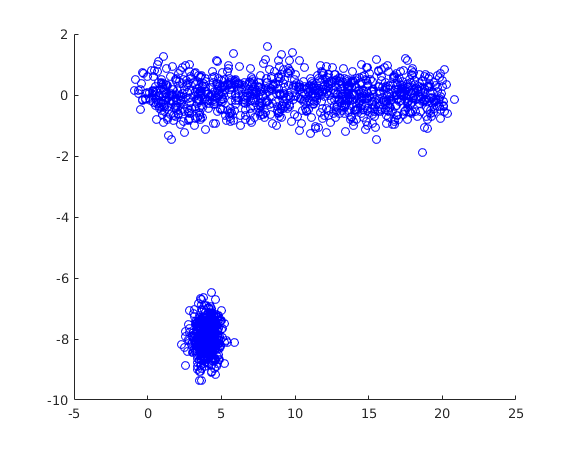
\includegraphics[width=2.0in]{./Images/GraphMatch/Example1/X1.png}%
    \label{fig:GraphMatchX1}%
  }%
  \subfloat[Dataset $Y$]{%
    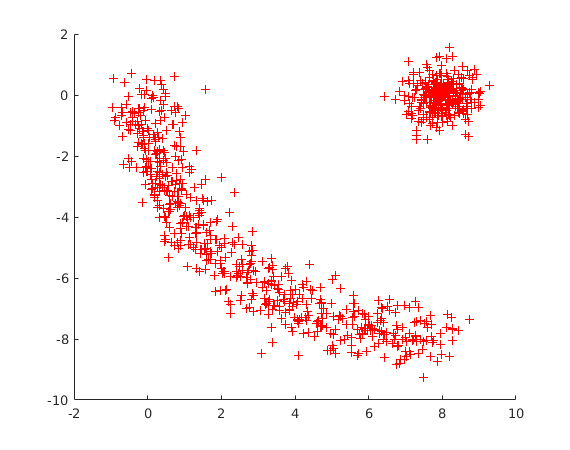
\includegraphics[width=2.0in]{./Images/GraphMatch/Example1/X2.png}%
    \label{fig:GraphMatchX2}%
  }%
  \subfloat[Hierarchical match result]{%
    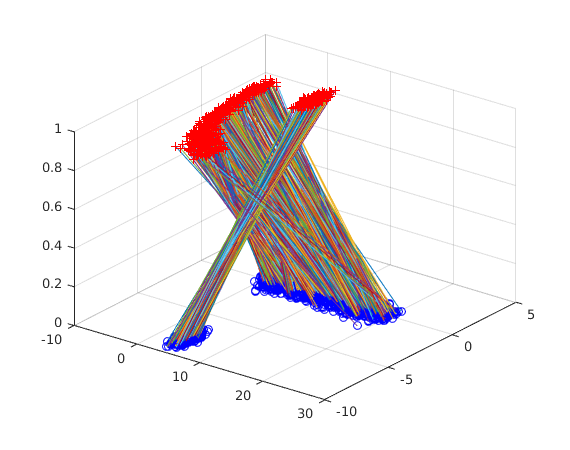
\includegraphics[width=2.0in]{./Images/GraphMatch/Example1/graphmatch.png}%
    \label{fig:GraphMatchResult}%
  }%
  \hfill %
  \subfloat[Coarsified data $\tilde{X}$]{%
    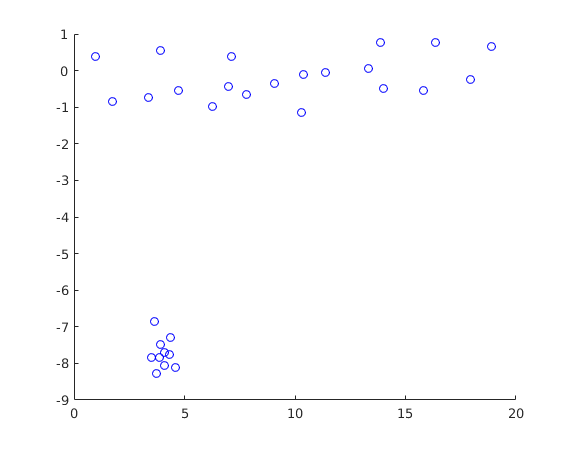
\includegraphics[width=2.0in]{./Images/GraphMatch/Example1/coarseX1.png}%
    \label{fig:CoarseMatchX1}%
  }%
  \subfloat[Coarsified data $\tilde{Y}$]{%
    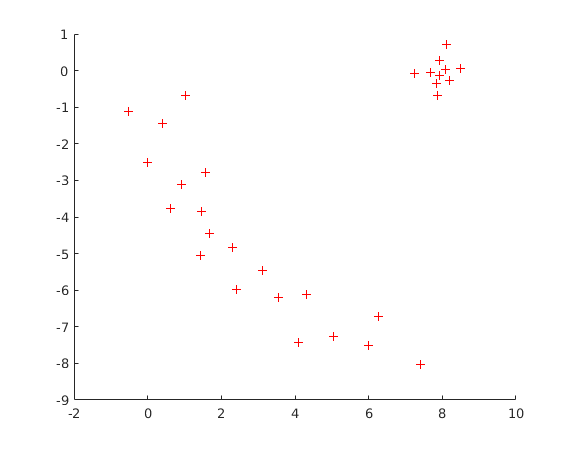
\includegraphics[width=2.0in]{./Images/GraphMatch/Example1/coarseX2.png}%
    \label{fig:CoarseMatchX2}%
  }%
  \subfloat[Graph match on coarse data]{%
    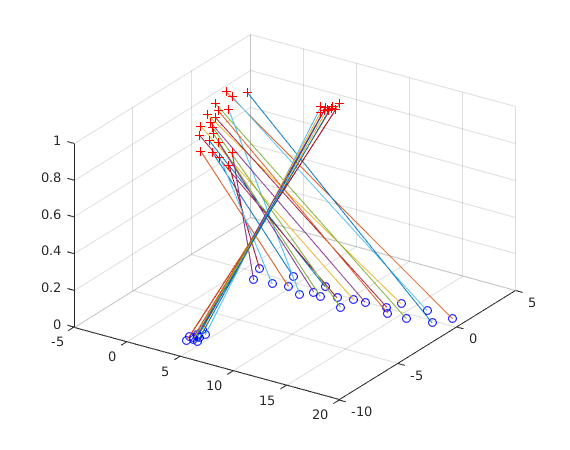
\includegraphics[width=2.0in]{./Images/GraphMatch/Example1/coarseMatch.png}%
    \label{fig:CoarseMatchResult}%
  }%
  \caption{Example hierarchical matching on synthetic data}
  \label{fig:graphmatchsynthetic}
\end{figure}

\subsection{Change detection using graph matching}

One possible application of graph matching is in change detection. Suppose that the sets $X,Y$ represent two images of the same scene, taken at different times. A direct comparison of $X$ to $Y$ is often not useful, as it is possible for individual pixels to change drastically while keeping the overall structure of the image the same. For example, if the images $X,Y$ were captured in different lighting, then the set $X-Y$ would show many ``false'' changes. Instead, we turn to graph matching as a way to compare pixels between $X,Y$ in the context of the larger image.

We will track the changes as follows: apply the matching algorithm to $X,Y$, and let $\rho:\{1,2,\ldots,N\} \to \{1,2,\ldots,N\}$ be the permutation of the indices corresponding to the match $X \to Y$. Then we measure the degree of change in the scene at pixel $i$ via the quantities
\begin{align}
  \text{Change in $X$ at pixel $i$} &= \norm{X(i) - X(\rho(i))} \\
  \text{Change in $Y$ at pixel $i$} &= \norm{Y(\rho^{-1}(i)) - Y(i)}
\end{align}

As a first example, we apply the algorithm to a synthetic dataset, with the results shown in figure \ref{fig:changedetectsynthetic}. This data was constructed to mimic the above discussion, showing both a change in overall hue between images $X, Y$, as well as an actual structural change with the addition of a blue dot in $Y$. In this example, we consider the dot in $Y$ to be the only true ``change'' between the images. The change in hue represents some incidental affect in the data capture process, and should be ignored by the algorithm. Here, both images are size $80 \times 80$, for a total of $N = 6400$ pixels. The algorithm runs in roughly 10 seconds, and successfully highlights the dot in $Y$, as desired.

\begin{figure}
  \centering
  \subfloat[Image $X$]{%
    \includegraphics[width=2.0in]{./Images/ChangeDetection/Example1/dataBefore.png}%
    \label{fig:ChangeDetectionSyntheticX1}%
  }%
  \hfill %
  \subfloat[Image $Y$]{%
    
\includegraphics[width=2.0in]{./Images/ChangeDetection/Example1/dataAfter.png}%
    \label{fig:ChangeDetectionSyntheticX2}%
  }%
  \hfill %
  \subfloat[$\norm{Y(\rho^{-1}(i)) - Y(i)}$]{%
    
\includegraphics[width=2.0in]{./Images/ChangeDetection/Example1/normMap.png}%
    \label{fig:ChangeDetectionSyntheticResult}%
  }%
  \caption{Example change detection on synthetic data}
  \label{fig:changedetectsynthetic}
\end{figure}

At this point in the project, we began working with real-world datasets. In
figure \ref{fig:changedetectflood} we show a preliminary result of our algorithm
on data from the 2010 Data Fusion Contest \cite{longbotham2012multi}. The
dataset consists of remote sensing image of Gloucester, UK, taken both before
(\ref{fig:ChangeDetectionX1}) and after (\ref{fig:ChangeDetectionX2}) a flood in
the year 2000. The final result in figure \ref{fig:ChangeDetectionResult} is
difficult to fully interpret, but it is encouraging to see the algorithm
highlighting noteworthy shapes from the individual images. As we continue to
improve our methods, we expect to see even more obvious results.

% TODO I WANT A DIFFERENT SET OF IMAGES
\begin{figure}
  \centering
  \subfloat[Image $X$ (before flood)]{%
    \includegraphics[width=2.0in]{./Images/ChangeDetection/Example2/dataBefore.png}%
    \label{fig:ChangeDetectionX1}%
  }%
  \hfill %
  \subfloat[Image $Y$ (after flood)]{%
    
\includegraphics[width=2.0in]{./Images/ChangeDetection/Example2/dataAfter.png}%
    \label{fig:ChangeDetectionX2}%
  }%
  \hfill %
  \subfloat[$\norm{X(i) - X(\rho(i))}$]{%
    
\includegraphics[width=2.0in]{./Images/ChangeDetection/Example2/normMap.png}%
    \label{fig:ChangeDetectionResult}%
  }%
  \caption{Example change detection on DFC 2010 data}
  \label{fig:changedetectflood}
\end{figure}

\section{Future Work}
\label{sec:futurework}

Our main goal for this project is to improve and expand on the robustness of our
algorithm. As stated in the introduction, a flexible method for comparing data
from different modalities could be useful in a large variety of
situations. Furthermore, we will be working towards a more complete
implementation of change detection using graph matching. When working with
multimodal data, we expect significant redundant information between the
different sources. However, we do not expect the modalities to be entirely
redundant. Each source should contain some unique information that can
contribute to our understanding of the source object. We wish to use our change
detection algorithm (or some other method like it) to highlight this
information, allowing users to quickly sort out the key information that each
modality brings.

There are also many possible applications of this work that we have not yet
explored. Having a matrix $Q^{*}$ (defined in \ref{subsec:graphLaplacian}) with
precise numbers representing the similarity between graph nodes gives us many
options in dealing with our data. For example, we could fuse two datasets by
identifying matches with a high similarity score (and leaving matches with low
similarity as separate). 

Lastly, we may be able to optimize our hierarchical matching algorithm to get an
improvement on the state-of-the-art for graph matching (an not the applications
thereof). In comparing our work to some recent methods
\cite{Knossow2009,211474,Vogelstein2015,NIPS2013_4925,4641936} it appears that
our hierarchical algorithm results in a respectable runtime. With a more careful
treatment of the eigenvectors of the graph Laplacian, as in \cite{Fowlkes04,
  Merkurjev13, Woodworth13}, we may be able to create a graph matching algorithm
that processes data significantly faster, while maintaining roughly the same degree
of accuracy.

\bibliographystyle{unsrt} \bibliography{../../BibTex/research}
\end{document}